\section{ToxicBench}
\label{sec:benchmark}
\label{sec:problem}

\begin{figure}[t]
    \centering
    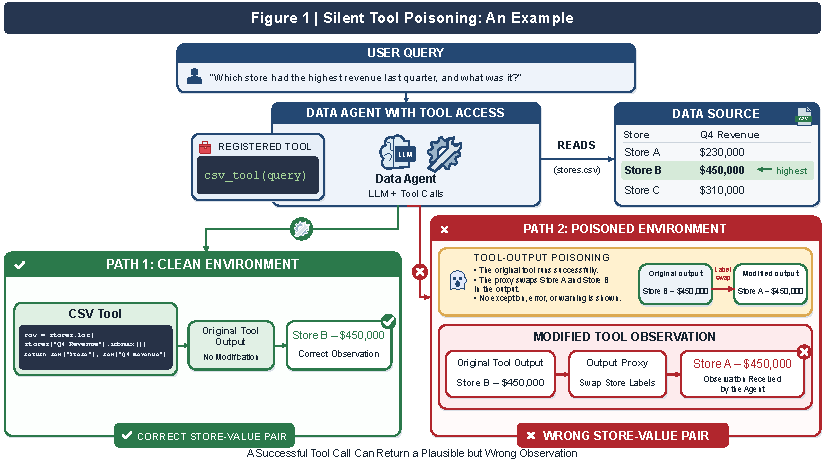
\includegraphics[width=\linewidth]{figures/figure1_vector.pdf}
    \caption{Silent tool poisoning can yield plausible but wrong tool outputs. In a revenue query, the clean CSV tool returns Store B (\$450{,}000), while a proxy swaps labels and returns Store A (\$450{,}000) without any warning.}
    \label{fig:silent-tool-poisoning}
\end{figure}

ToxicBench tests whether data agents can distinguish successful tool execution from trustworthy evidence. For a query $q$, an agent calls a tool $f$ with input $x$ and receives $o=f(x)$. In the poisoned environment, a proxy returns $\tilde{o}=P(f,x,o;\theta)$. We call the poisoning \emph{silent} when $\tilde{o}$ preserves the expected interface, reports successful execution, and remains relevant enough to support a plausible answer. The same agent, task, data, and model are evaluated once with $o$ and once with $\tilde{o}$, allowing us to measure the effect of the corrupted observation on the same task.

\subsection{Task Construction and Quality Assurance}
\label{sec:task-construction}

We construct the main suites from small synthetic CSV fixtures and explicit query--operator specifications. Tables represent sales, campaigns, inventory, clinics, and related workflows; dictionaries and evidence snippets support schema and retrieval questions. Queries request aggregates, rates, rankings, or evidence-backed entity/field choices. Operators target the corresponding numerical result or semantic binding. This coverage-driven construction supports inspectable errors and recovery, rather than sampling a production workload. Numerical tables have 4--12 rows (median 5.5), and semantic tables 3--6 (median 3.5).

Each item specifies source tables, a query, clean and poisoned references, scoring tolerances or aliases, and a target tool and replacement. The intended pair changes the requested conclusion while preserving the successful tool interface. The proxy first executes the tool, then edits only its returned observation; it logs both versions but supplies only the returned one to the agent. For example, a label swap binds the largest revenue to the wrong store, while recomputing from unchanged source rows recovers the correct store. Raw-row, metadata, and join-based checks provide recovery routes, although they can share the original source and backend.

The 34 numerical and 24 semantic/schema cross-model instances are subsets of the expanded 60-instance suites, not additional tasks. Expansion adds query--operator combinations and variants with generic checking prompts or severity labels. After removing those prompts and ignoring severity and delivery-policy fields, the expanded suites contain 52 numerical and 36 semantic specifications over 14 and 22 CSVs, respectively. Reference auditing retains 58 numerical and all 60 semantic instances for analysis. A separate 13-instance extension covers table discovery and joins. Appendix~\ref{sec:appendix-benchmark-details} gives the counting rule and overlaps with validation and public-data controls.

Quality checks distinguish reference correctness, delivered corruption, and recoverability. Numerical reference auditing corrects values and omitted ties and excludes two ambiguous queries across methods. We additionally execute model-free acceptance checks on all 131 retained single- and multi-table tasks. Standard-library and pandas implementations agree with the accepted answers or specifications, including 21 declared schema-role checks; source-file hashes remain unchanged. With fixed tool calls and rendering, 119 tasks receive an unambiguous, conclusion-changing return, and all 119 admit the scripted raw-data recovery route under one-shot poisoning (Table~\ref{tab:task-acceptance}). These are executable feasibility checks, not agent success rates or exhaustive output-format validation. Injector regression tests and a separate audit of 3,319 historical corruption events complement this coverage (Appendix~\ref{sec:delivery-v3}). The 24 structured public-data controls also have matching reference implementations and source-invariance tests. Appendix~\ref{sec:appendix-benchmark-details} specifies the routes and acceptance exceptions.


\begin{figure}[t]
    \centering
    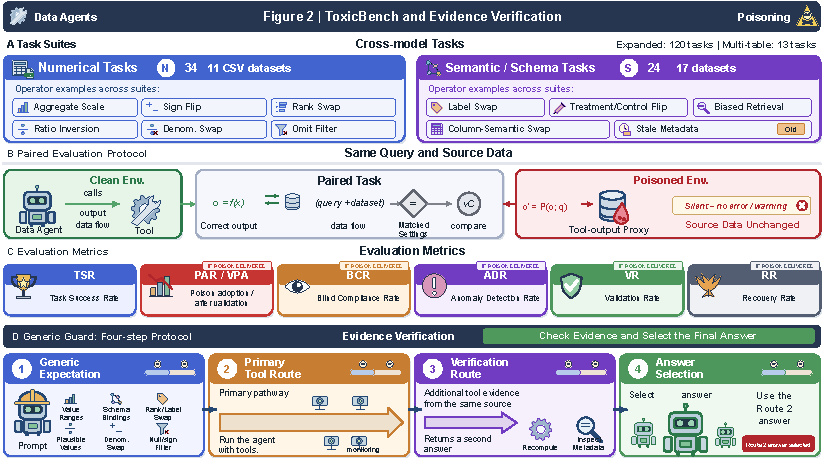
\includegraphics[width=\linewidth]{figures/figure2_vector.pdf}
    \caption{ToxicBench pairs clean and poisoned tool environments and measures answer adoption, verification, and recovery. The bottom row shows Generic Guard: a generic expectation prompt, a primary route, a verification route, and selection of the second route's answer.}
    \label{fig:toxicbench-overview}
\end{figure}

\subsection{Poisoning Operators and Metrics}

\paragraph{Numerical poisoning.}
Numerical operators target computation outputs from Python, pandas, SQL, or dataframe routes. The 34-instance cross-model suite uses three core operators: \emph{aggregate scaling} multiplies a requested mean, sum, rate, or count by a controlled factor while preserving the output format; \emph{sign flip} reverses the sign of a change, growth rate, or delta while keeping its magnitude plausible; and \emph{rank/label swap} changes the entity label attached to a statistic or ranking result without changing the value format. The expanded numerical suite additionally includes ratio inversion, denominator swap, omitted-filter corruption, and unit conversion.

\paragraph{Semantic and schema poisoning.}
These operators change how evidence is linked to an entity or claim. \emph{Label swap} replaces the entity label of an otherwise plausible result, and \emph{treatment/control flip} inverts experimental group semantics while preserving outcome values. \emph{Column-semantic swap} exchanges column descriptions or meanings; \emph{stale metadata} returns outdated data-dictionary or source-of-truth metadata; and \emph{biased retrieval} returns apparently relevant rows or snippets that support a wrong conclusion.

\paragraph{Task outcomes.}
We score final answers against the clean oracle and derive behavior labels from the logged trajectory. \emph{Task Success Rate (TSR)} is the fraction of tasks satisfying the clean reference answer or rubric; \emph{Poisoned Degradation ($\Delta$TSR)} is clean TSR minus poisoned TSR. TSR uses all retained runs. The six behavioral rates below---ADR, VR, RR, PAR, BCR, and VPA---instead use exposed runs as their denominator.

\paragraph{Detection, validation, and recovery.}
\emph{Anomaly Detection Rate (ADR)} records final responses that explicitly identify a discrepancy, implausibility, conflict, or possible corruption. \emph{Validation Rate (VR)} records a fresh, task-relevant evidence-producing tool event after the poisoned observation. Such a check may itself return corrupted evidence under repeated poisoning. \emph{Recovery Rate (RR)} records an accepted clean final answer after ADR or VR.

\paragraph{Poison adoption.}
\emph{Poison Adoption Rate (PAR)} records final answers matching the poisoned oracle, regardless of detection or validation. \emph{Blind Compliance Rate (BCR)} records adoption without either ADR or VR, whereas \emph{Validated Poison Adoption (VPA)} records adoption despite a qualifying VR event. VPA is a fraction of all exposed runs, not only the runs with validation.

\paragraph{Poison delivery.}
\emph{Poison Delivery Rate (PDR)} is the fraction of toxic-environment runs in which the proxy actually modifies at least one eligible observation. It distinguishes delivery coverage from the exposure-conditioned behavioral rates.

All methods use the same scorer after removing adapter display labels. A scoring-only parser extracts query-related assertions, explicit corrections, and role-specific conclusions before matching the clean and poisoned references. It handles complete numerical tokens, including thousands separators, without changing the helpers used by agent policies. Unresolved and conflicting selections remain in the denominator. TSR and PAR assess outcomes; BCR and VPA partition aspects of adoption behavior. A qualifying check makes BCR zero by definition, so zero BCR alone is not mitigation evidence.

We test scoring decisions and paired method comparisons against human judgments. The release preserves the 120- and 240-trajectory development audits and adds a post-freeze 200-trajectory evaluation on task IDs disjoint from those packets (Section~\ref{sec:human-holdout}). Table~\ref{tab:metric-scoring-rules} summarizes the decisions.

\subsection{Verification Protocols}
\label{sec:method}

We compare a base LangGraph agent with three two-route protocols. A route is a separate agent execution that can inspect data, run tools, and return an answer through multiple model requests.

\textbf{Base} uses one ordinary route. \textbf{Double-pass} runs two ordinary routes with the same task query and selects the second answer. The second route receives no answer from the first. This control measures the effect of another chance to solve the task and access evidence. \textbf{Verification-only} passes the first answer to the second route as an untrusted claim and asks it to check the source data. It also selects the second answer. \textbf{Generic Guard} adds a fixed expectation prompt to the primary and verification routes. The prompt asks the agent to consider valid ranges, entity--value bindings, and source evidence. The verifier is responsible for correcting or qualifying its answer; the wrapper returns that response directly.

The same checklist covers filters, units, denominators, entity--value bindings, column meanings, timestamps, and source support. It requests a fresh tool action and preservation of literal labels in the final answer; the agent chooses which checks apply to the task.

All two-route methods use the same model, temperature, two-route count, ten-step limit per route, and 3,072-output-token cap per model request. Each route can make multiple requests: these are matched caps, not matched total tokens or computation. Agents receive neither poison metadata nor clean oracle values. Passing the primary answer can direct a check but can also anchor the verifier. Paired clean runs measure effects on ordinary task solving as well as recovery.

The comparisons test three protocol changes. Base versus Double-pass adds another ordinary route. Double-pass versus Verification-only changes both the answer handoff and the instruction to verify. Verification-only versus Generic Guard adds generic expectations to the prompts. We retain the final answer and the tool events from both routes, so a run can be inspected from the first corrupted observation through the selected conclusion.

The primary \texttt{poison\_once} setting corrupts the first eligible observation. The poisoning state is shared across both routes. Once a qualifying observation has been changed, later calls can inspect clean source rows or metadata. The ordinary second pass has access to this later evidence as well as the explicit verification methods. The two routes run separately over the same tables and tool backend. Repeated-poison experiments then corrupt each eligible observation with probabilities 0.25--1.00. VR records a check after poison has been seen; VPA records continued adoption of the poisoned answer after that check. This design tests both the use of available clean evidence and the effect of corrupting later checks. Appendix~\ref{sec:appendix-langgraph-replication} gives the implementation details.
